\chapter{Attack Simulation}
\label{cap:attacksimulations}

% point out comparison better! check whole chapter

The reliability based \ac{CMA-ES} is the only attack which is claimed to have a linear increasing time consumption for successful attacks on \xpufs that grow linear in their number of used \apufs, as explained in Sec. \ref{sec:essentialattacks}.
Successfully attacked means to building a model that can predict $80 \%$ of the challenges from a test set that contains randomly chosen challenges correct.
The implementation of the \ac{CMA-ES} attack, how it is based on reliability, and the \apuf simulation is explained in Chap. \ref{cap:simulationdesign}.
As the attack is based on the unreliability of challenges first the dependency between the number of \acp{MV} and the number of collected unreliable challenges is studied.
After that the success of the \ac{CMA-ES} attack on \mpufs is evaluated, since they are used to build the \mxpuf.
Finally the \ac{CMA-ES} attack is applied to \mxpufs of different size to study whether \ac{MV} can prevent the attack through enabling large \mxpufs. 

% same configuration as for stability simulation, repeat and ref
% ref to machine learning design
%========================================

\section{Detection of Unreliable Challenges}
\label{sec:detectionofunreliablechallenges}

For the reliability based \ac{CMA-ES} attack on \apufs it is crucial to find challenges which evaluate differently at multiple evaluations as explained in Sec. \ref{sec:reliability}.
To find these challenges and their reliability $\gls{h}$ every challenge $\gls{c}$ of a set will be evaluated $\gls{j}$ times.
After that the reliability $\gls{h}$ will be computed for every challenge by \ref{equ:reliability}.
Do not get confused with the notions stability and reliability as the definition of reliability differs for the \ac{CMA-ES} attack, as explained in Sec. \ref{sec:reliability}.

When using \ac{MV} to increase the stability of the \apuf finding challenges with lower reliability becomes more difficult.
Hence Fig. \ref{fig:cmamajorityvotemeasurementrelation} shows the relation between the increase of votes $\gls{m}$ and the decrease of found challenges which lowered reliability $\gls{h}$.
In this case a lowered reliability is already reached if a challenge $\gls{c}$ evaluates one or multiple times different to the rest of the evaluations for $\gls{j}$ number of evaluations and is called unreliable. % in contrast to term unstable.
There are four line graphs for the different numbers of evaluations $\gls{j}$.

\begin{figure}[ht]
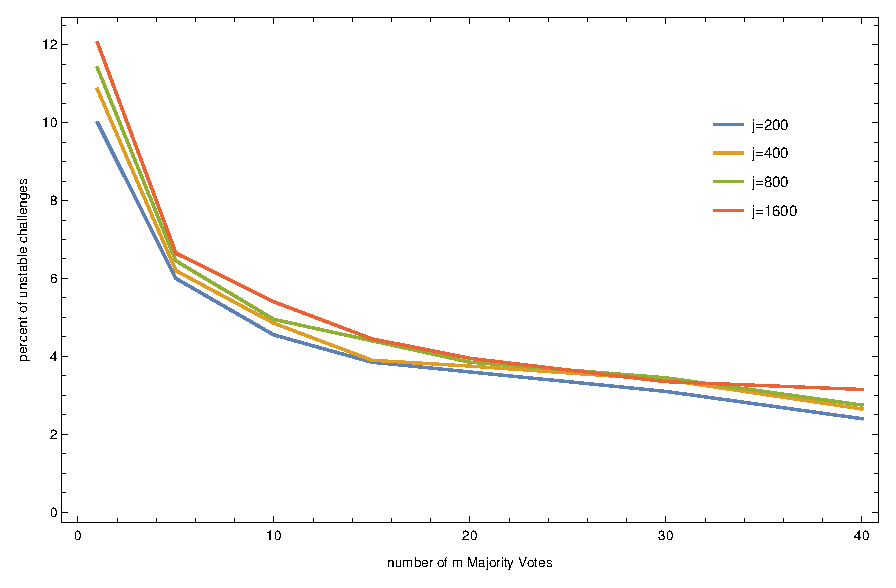
\includegraphics[width=1.00\textwidth]{images/mv-measurements-unstableChallenges.eps}
% \noindent\includegraphics[width=1.00\textwidth, height=3cm, draft]{example-image-a}
\caption[Proportion of unreliable challenges]{Proportion of unreliable challenges for different values of $\gls{m}$ \acp{MV}. The different line graphs represent the $\gls{j}$ number of evaluations $200, 400, 800, 1600$. The slight distance between the graphs in the beginning shows the very little increase of found unreliable challenges with increasing number of evaluations $\gls{j}$ and how this gap resolves with introducing of \ac{MV}.}
\label{fig:cmamajorityvotemeasurementrelation}
\end{figure}

% Old and wrong: The raising gradient of all four graphs could lead to the same assumption display the subsiding impact of \ac{MV} with rising $\gls{m}$ as explained in Sec. \ref{sec:stabilityimprovementbymajorityvote}.
The raising gradient of all four graphs could lead to the same assumption of the subsiding impact of \ac{MV} with rising $\gls{m}$ as explained in Sec. \ref{sec:stabilityimprovementbymajorityvote}.
However the linear course of the graph shown by the logarithmic Fig. \ref{fig:cmamajorityvotemeasurementrelationloglog} suggest that this is not the case and supports the result of Sec. \ref{sec:stabilityimprovementbymajorityvote}.

\begin{figure}[ht]
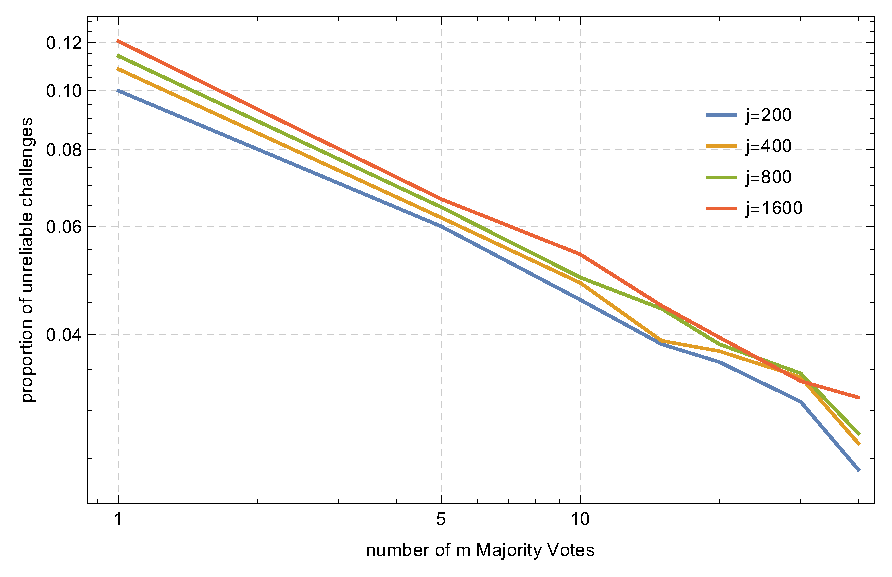
\includegraphics[width=1.00\textwidth]{images/mv-measurements-unstableChallenges_loglog.eps}
% \noindent\includegraphics[width=1.00\textwidth, height=3cm, draft]{example-image-a}
\caption[Proportion of unreliable challenges logarithmic]{The line graphs show the proportions of unreliable challenges for different values of $\gls{m}$ \acp{MV} similar to Fig. \ref{fig:cmamajorityvotemeasurementrelation} yet in logarithmic scale. The linear course of the graphs suggest that there is no decline of the stability improving impact of \ac{MV} with increasing $\gls{m}$ used for \mpufs.}
\label{fig:cmamajorityvotemeasurementrelationloglog}
\end{figure}

The only slight difference between the graphs in both figures show that increasing the number of evaluation $\gls{j}$ does not necessarily provides more challenges with lowered reliability $\gls{h}$.
Without \ac{MV} there is a little increase of found challenges with lowered reliability $\gls{h}$.
Though with applying \ac{MV} this increase disappears with growing $\gls{m}$.

%========================================

\section{\apufs vs. \mpufs}
\label{sec:arbitervsmajorityarbiter}

This section describes the results of the simulation used to study the success of the \ac{CMA-ES} attack, explained in Sec. \ref{sec:cma-esdesign}, on \mpufs.
Through the comparison with the success of the attack on \apuf the impact of \ac{MV} can be evaluated.
The \apuf used for the simulation has $\gls{n} = 32$ stages.
For the attack a training set of $10000$ \acp{CRP} and a number of evaluation times of $\gls{j} = 100$ were used.
Since the \ac{CMA-ES} attack not always approximates to a model, which performs well on challenges of the test set, it has to be restarted.
The number of needed starts of the attack till a desired model has been approximated is called number of attack executions.
A model produced by the attack is defined to perform well if it evaluates $80 \%$ of the $10000$ \acp{CRP} of the test set correct.
Both test set and training set are independent randomly chosen sets of challenges $\gls{c}$.
The exit criteria sigma of the \ac{CMA-ES} attack as explained in Sec. \ref{sec:cma-esdesign} is set to $0.2$ and stops the attack despite if the attack approximates to a model which performs well on the test set or not.
For a growing number of \ac{MV} $\gls{m}$ there is an increase of needed executions of the attack to approximate to a model which performs well on the test set, as shown in Fig \ref{fig:cmasingleattackcorrelation}.
The growing gradient of the graph shows the growing exponential increase of needed attack executions to gain well performing models.
From $\gls{m} = 80$ \acp{MV} on the gradient of the graph is greater than $1$.
Hence the slope of the number of attack executions is greater than the polynomial degree $1$.

\begin{figure}[ht]
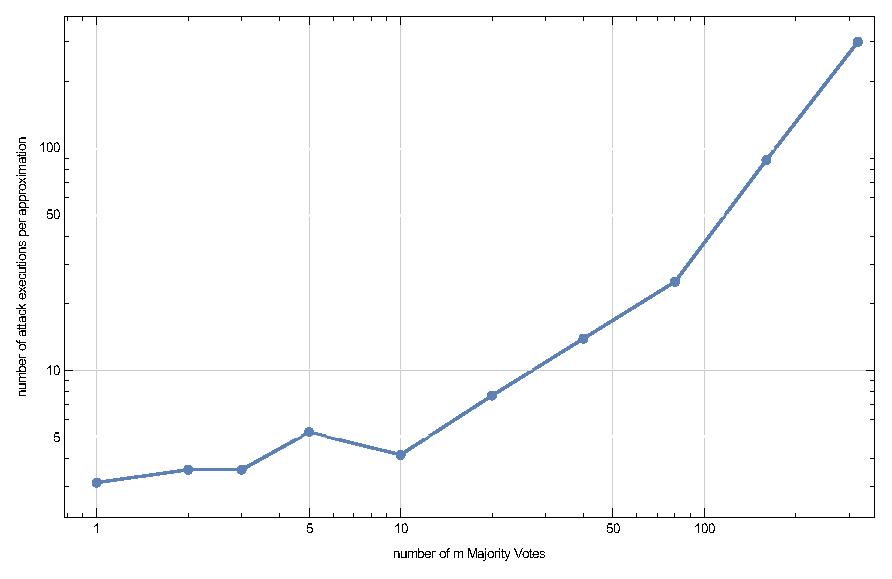
\includegraphics[width=1.00\textwidth]{images/single-mv-classification-cma-attack-correlation.eps}
% \noindent\includegraphics[width=1.00\textwidth, height=3cm, draft]{example-image-a}
\caption[Needed \acs{CMA-ES} attack executions for \mpufs]{Number of attack executions per approximation to a well performing model. A well performing model evaluates $80 \%$ of the $10000$ test set \acp{CRP} correct. The rising gradient of the graph shows the growing exponential increase of the number of attack executions.}
\label{fig:cmasingleattackcorrelation}
\end{figure}

Apart from the increasing number of attack executions the performance of the computed models decreases with the growth of $\gls{m}$, as shown in Fig. \ref{fig:cmasingleattackcorrectness}.
The graph displays how the proportion of correct evaluated challenges $\gls{c}$ of the test set lowers linear with a linear rise of the number of \ac{MV} $\gls{m}$.
This indirect correlation implies that with growing number of \ac{MV} $\gls{m}$ the proportion of the correct evaluated challenges $\gls{c}$ of the test set decreases for well performing models build by the \ac{CMA-ES} attack.
The values of both Fig. \ref{fig:cmasingleattackcorrelation} and \ref{fig:cmasingleattackcorrectness} are average values of minimum $10$ well performing models except for the last value of $m = 320$ that required $2000$ attack executions to gain $5$ well performing models.
\todo{maybe measure m=320 with additional 2000 executions}

\begin{figure}[ht]
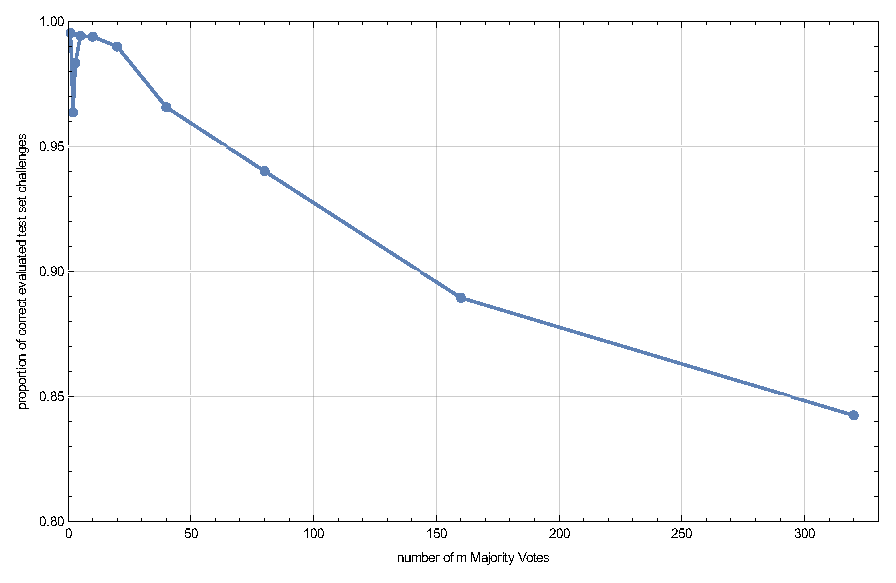
\includegraphics[width=1.00\textwidth]{images/single-mv-classification-cma-attack-correctness.eps}
% \noindent\includegraphics[width=1.00\textwidth, height=3cm, draft]{example-image-a}
\caption[Proportion of correct evaluated test set challenges of a model approximated by the \acs{CMA-ES} attack]{Proportion of correct evaluated test set \acp{CRP} of a well performing model build by an \ac{CMA-ES} attack. The linear decrease of the graph shows the decrease of the proportion of correct evaluated challenges $\gls{c}$ by a well performing model. The values used are average values of minimum $10$ well performing model or at least $2000$ attack executions.}
\label{fig:cmasingleattackcorrectness}
\end{figure}

%========================================

\section{\acs{XOR} \apufs vs. Majority \acs{XOR} \apufs}
\label{sec:xorarbitervsmajorityxorarbiter}


\xpuf to unstable with growing k




%========================================

